\setcounter{section}{0}
\section{Trắc nghiệm}
\begin{enumerate}[label=\bfseries Câu \arabic*:]
	\item \mkstar{1}
	
	{Chọn đáp án đúng nhất. Trường hợp nào sau đây có công cơ học?
		\begin{mcq}
			\item Khi có lực tác dụng vào vật. 
			\item Khi có lực tác dụng vào vật và vật chuyển động theo phương vuông góc với lực. 
			\item Khi có lực tác dụng vào vật và vật đứng yên. 
			\item Khi có lực tác dụng vào vật và vật chuyển động. 
		\end{mcq}
	}
	
	\hideall
	{		\textbf{Đáp án: D.}
		
		
	}
	\item \mkstar{1}
	
	
	{Công thức tính công cơ học khi lực $F$ làm vật dịch chuyển một quãng đường $s$ theo hướng của lực là
		\begin{mcq}(2)
			\item $A=\dfrac{F}{s}$. 
			\item $A=Fs$.
			\item $A=\dfrac{s}{F}$. 
			\item $A=F-s$. 
		\end{mcq}
	}
	
	\hideall
	{		\textbf{Đáp án: B.}
		
		Công thức tính công cơ học khi lực $F$ làm vật dịch chuyển một quãng đường $s$ theo hướng của lực là $A=Fs$.
		
	}
	\item \mkstar{1}
	
	
	{Trong các phát biểu sau, phát biểu nào đúng với định luật về công?
		\begin{mcq}
			\item Các máy cơ đơn giản đều cho ta lợi về công. 
			\item Không một máy cơ đơn giản nào cho ta lợi về công. 
			\item Không một máy cơ đơn giản nào cho ta lợi về lực. 
			\item Không một máy cơ đơn giản nào cho ta lợi về đường đi. 
		\end{mcq}
	}
	
	\hideall
	{\textbf{Đáp án: B.}
		
		Không một máy cơ đơn giản nào cho ta lợi về công. Được lợi bao nhiêu lần về lực thì thiệt bấy nhiêu lần về đường đi và ngược lại.
		
	}
	\item \mkstar{1}
	
	
	{Theo chương trình Vật lý THCS, có bao nhiêu loại máy cơ đơn giản?
		\begin{mcq}(4)
			\item 1. 
			\item 2. 
			\item 3. 
			\item Rất nhiều. 
		\end{mcq}
	}
	
	\hideall
	{\textbf{Đáp án: C.}
		
		Có 3 loại máy cơ đơn giản: mặt phẳng nghiêng, đòn bẩy, ròng rọc.
		
		
	}
	\item \mkstar{1}
	
	
	{
		Trong trường hợp nào dưới đây \textbf{không} có công cơ học?
		\begin{mcq}
			\item Một người đang kéo một vật chuyển động. 
			\item Hòn bi đang chuyển động thẳng đều trên mặt sàn nằm ngang coi như tuyệt đối nhẵn. 
			\item Một lực sĩ đang nâng quả tạ từ thấp lên cao. 
			\item Máy xúc đất đang làm việc. 
		\end{mcq}
	}
	
	\hideall
	{\textbf{Đáp án: B.}
		
		Hòn bi đang chuyển động thẳng đều trên mặt sàn nằm ngang coi như tuyệt đối nhẵn không có công cơ học.
		
	}
	
	\item \mkstar{1}
	
	
	{Trong các phát biểu sau, phát biểu nào \textbf{sai}?
		\begin{mcq}
			\item Ròng rọc cố định chỉ có tác dụng đổi hướng của lực và cho ta lợi về công. 
			\item Ròng rọc động cho ta lợi hai lần về lực, thiệt hai lần về đường đi.
			\item Mặt phẳng nghiêng cho ta lợi về lực, thiệt về đường đi. 
			\item Đòn bẩy cho ta lợi về lực, thiệt về đường đi.
		\end{mcq}
		
	}
	
	\hideall
	{\textbf{Đáp án: A.}
		
		Ròng rọc cố định chỉ có tác dụng đổi hướng của lực và không cho ta lợi về công. 
		
	}
	\item \mkstar{1}
	
	
	{Công suất là
		\begin{mcq}
			\item công thực hiện được trong một giây. 
			\item công thực hiện được trong một ngày. 
			\item công thực hiện được trong một giờ.
			\item công thực hiện được trong một đơn vị thời gian. 
		\end{mcq}
		
	}
	
	\hideall
	{\textbf{Đáp án: D.}
		
		
	}
	
	\item \mkstar{1}
	
	
	{Biểu thức tính công suất là
		\begin{mcq}(4)
			\item $\calP = \dfrac{A}{t}$.
			\item $\calP = At$.
			\item $\calP= \dfrac{t}{A}$.
			\item $\calP = \dfrac{A}{t^2}$.
		\end{mcq}
	}
	
	\hideall
	{	\textbf{Đáp án: A.}
		
	}
	\item \mkstar{1}
	
	
	{Đơn vị của công suất là
		\begin{mcq}(2)
			\item W.
			\item kW.
			\item J/s.
			\item Tất cả đều đúng.
		\end{mcq}
	}
	
	\hideall
	{\textbf{Đáp án: D.}	
		
	}
	\item \mkstar{1}
	
	
	{Vật có cơ năng khi
		
		\begin{mcq}(2)
			\item vật có khả năng sinh công.	
			\item vật có khối lượng lớn.	
			\item vật có tính ì lớn.	
			\item vật đứng yên.	
		\end{mcq}
		
	}
	
	\hideall
	{\textbf{Đáp án: A.}
		
		Vật có cơ năng khi vật có khả năng sinh công.	
		
	}
	\item \mkstar{1}
	
	
	{Thế năng hấp dẫn phụ thuộc vào những yếu tố nào?
		
		\begin{mcq}(2)
			\item Khối lượng.
			\item Trọng lượng riêng.	
			\item Khối lượng và độ cao.	
			\item Khối lượng và vận tốc.	
		\end{mcq}
		
	}
	
	\hideall
	{\textbf{Đáp án: C.}
		
	}
	\item \mkstar{1}
	
	
	{Phát biểu nào sau đây đầy đủ nhất khi nói về sự chuyển hóa cơ năng?
		
		\begin{mcq}
			\item Động năng có thể chuyển hóa thành thế năng.	
			\item Thế năng có thể chuyển hóa thành động năng.	
			\item Động năng và thế năng có thể chuyển hóa lẫn nhau, cơ năng không được bảo toàn.	
			\item Động năng và thế năng có thể chuyển hóa lẫn nhau, cơ năng được bảo toàn.
		\end{mcq}
		
	}
	
	\hideall
	{\textbf{Đáp án: D.}
		
	}
	\item \mkstar{2}
	
	
	{Một người dùng một cần cẩu để nâng một thùng hàng có khối lượng 2500 kg lên độ cao 12 m từ mặt đất. Tính công thực hiện được trong trường hợp này.
		
		\begin{mcq}(4)
			\item $\SI{300}{kJ}$.
			\item $\SI{250}{kJ}$.	
			\item $\SI{2.08}{kJ}$.	
			\item $\SI{300}{J}$.	
		\end{mcq}
		
	}
	
	\hideall
	{\textbf{Đáp án: A.}
		
		Công thực hiện được là
		$$A=10mh=\SI{300}{kJ}$$
	}
	\item \mkstar{2}
	
	
	{Một đầu máy xe lửa kéo các toa xe bằng lực $F=\SI{7500}{N}$. Công của lực kéo là bao nhiêu khi các toa xe chuyển động được quãng đường $s=\SI{8}{km}$?
		
		\begin{mcq}(4)
			\item $\SI{60000}{kJ}$.	
			\item $\SI{60}{kJ}$.	
			\item $\SI{60000}{J}$.
			\item Kết quả khác.	
		\end{mcq}
		
	}
	
	\hideall
	{\textbf{Đáp án: A.}
		
		Công thực hiện được là
		$$A=10mh=\SI{60000}{kJ}$$
	}
	\item \mkstar{2}
	
	
	{Con ngựa kéo xe chuyển động đều với vận tốc $\SI{9}{km/h}$. Lực kéo là $200\ \text N$. Công suất của ngựa nhận giá trị nào sau đây?
		
		\begin{mcq}(4)
			\item $\SI{1500}{W}$.
			\item $\SI{500}{W}$.
			\item $\SI{1000}{W}$.	
			\item $\SI{250}{W}$.
		\end{mcq}
		
	}
	
	\hideall
	{\textbf{Đáp án: B.}
		
		Công suất là
		$$\calP = \dfrac{A}{t} = Fv=\SI{500}{W}$$
	}
	\item \mkstar{2}
	
	
	{Một máy cơ trong 1 giờ sản ra một công là $\SI{330}{kJ}$. Công suất của máy cơ này là
		
		\begin{mcq}(4)
			\item $\SI{92.5}{W}$.	
			\item $\SI{91.7}{W}$.	
			\item $\SI{90.2}{W}$.	
			\item $\SI{97.5}{W}$.	
		\end{mcq}
		
	}
	
	\hideall
	{\textbf{Đáp án: B.}
		
		Công suất là
		$$\calP = \dfrac{A}{t} = \SI{91.7}{W}$$
	}
	\item \mkstar{3}
	
	
	{Người ta dùng một mặt phẳng nghiêng để kéo một vật. Nếu không có ma sát thì công cần thiết là 125 J. Thực tế có ma sát nên công cần thiết là 175 J. Hiệu suất của mặt phẳng nghiêng trên là bao nhiêu?
		
		\begin{mcq}(4)
			\item $\SI{81.33}{\%}$.	
			\item $\SI{83.33}{\%}$.	
			\item $\SI{71.43}{\%}$.	
			\item $\SI{77.33}{\%}$.	
		\end{mcq}
		
	}
	
	\hideall
	{\textbf{Đáp án: C.}
		
		Hiệu suất:
		$$H=\dfrac{A_\text{ích}}{A_\text{toàn phần}} = \dfrac{A_F}{A_F + A_\text{ms}} =\SI{71.43}{\%} $$
	}
	\item \mkstar{3}
	
	
	{Một người đi xe đạp đều từ chân dốc đến đỉnh dốc cao 5 m. Dốc dài 40 m, biết lực ma sát cản trở chuyển động của xe có độ lớn là 20 N. Cả người và xe có khối lượng là $\SI{37.5}{kg}$. Công tổng cộng do người đó sinh ra là bao nhiêu?
		
		\begin{mcq}(4)
			\item 3800 J.	
			\item 4200 J.	
			\item 4000 J.	
			\item 2675 J.	
		\end{mcq}
		
	}
	
	\hideall
	{\textbf{Đáp án: D.}
		
		Công do người đó sinh ra:
		$$A=A_P + A_\text{ms} = 2675\ \text J$$	
	}
	\item \mkstar{3}
	
	
	{Một cái máy bơm dùng để bơm nước vào ao. Một giờ nó bơm được $\SI{1000}{m^3}$ nước lên cao 2 m. Biết trọng lượng riêng của nước là $\SI{10000}{N/m^3}$. Công suất của máy bơm là
		
		\begin{mcq}(4)
			\item $\SI{5}{kW}$.	
			\item $\SI{5200.2}{W}$.	
			\item $\SI{5555.6}{W}$.	
			\item $\SI{5650}{W}$.	
		\end{mcq}
		
	}
	
	\hideall
	{\textbf{Đáp án: C.}
		
		Công suất máy bơm:
		$$\calP = \dfrac{A}{t} = \dfrac{Ph}{t} = \dfrac{dVh}{t} = \SI{5555.6}{W}$$
	}
	\item \mkstar{4}
	
	
	{Người ta dùng vật B kéo vật A ($m_\text A = 10\ \text{kg}$) chuyển động đều đi lên mặt phẳng nghiêng.
		\begin{center}
			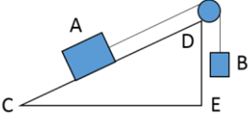
\includegraphics[scale=1]{../figs/VN10-2021-PH-TP0003-1.png}
		\end{center}
		Biết CD = 4 m, DE = 1 m. Bỏ qua ma sát, vật B có khối lượng bao nhiêu?
		\begin{mcq}(4)
			\item $\SI{4}{kg}$.	
			\item $\SI{2.5}{kg}$.	
			\item $\SI{1.5}{kg}$.
			\item $\SI{5}{kg}$.
		\end{mcq}
		
	}
	
	\hideall
	{\textbf{Đáp án: B.}
		
		Độ nghiêng của mặt phẳng nghiêng:
		$$\sin \alpha = \dfrac{\text{DE}}{\text{CD}} = 14,47^\circ$$
		
		Trọng lực tác dụng lên vật A theo phương mặt phẳng nghiêng:
		$$P_x=P_A \sin \alpha = 25\ \text N$$
		
		Vậy vật B phải có khối lượng là $m_\text B = \dfrac{P_B}{10} = \SI{2.5}{kg}$
	}
	
\end{enumerate}


\hideall
{
	\begin{center}
		\textbf{BẢNG ĐÁP ÁN}
	\end{center}
	\begin{center}
		\begin{tabular}{|m{2.8em}|m{2.8em}|m{2.8em}|m{2.8em}|m{2.8em}|m{2.8em}|m{2.8em}|m{2.8em}|m{2.8em}|m{2.8em}|}
			\hline
			1.D  & 2.B  & 3.B  & 4.C  & 5.B  & 6.A  & 7.D  & 8.A  & 9.D  & 10.A  \\
			\hline
			11.C  & 12.D  & 13.A  & 14.A  & 15.B  & 16.B  & 17.C  & 18.D  & 19.C  & 20.B  \\
			\hline
			
		\end{tabular}
	\end{center}
}
\section{Tự luận}
\begin{enumerate}[label=\bfseries Câu \arabic*:]
	\item \mkstar{1}
	
	{
		Phát biểu định nghĩa công cơ học. Viết biểu thức tính công cơ học.
	}
	
	\hideall{
		Thuật ngữ công cơ học chỉ dùng trong trường hợp có lực tác dụng làm vật chuyển dời.
		
		Công cơ học phụ thuộc vào 2 yếu tố: Lực tác dụng vào vật và quãng đường vật dịch chuyển.
		
		Công cơ học thường được gọi tắt là công.
		
		Công thức tính công khi lực $F$ làm vật dịch chuyển một quãng đường $s$ theo phương của lực:
		$$A=Fs$$
	}
	
	\item \mkstar{1}
	
	{Phát biểu định nghĩa công suất. Viết biểu thức tính công suất.}
	
	\hideall{
		Công suất được xác định bằng công thực hiện trong một đơn vị thời gian.
		
		Biểu thức tính công suất:
		$$\calP = \dfrac{A}{t}$$
	}
	\item \mkstar{1}
	
	
	{Phát biểu nội dung của sự chuyển hóa và bảo toàn cơ năng.
	}
	
	\hideall
	{Động năng có thể chuyển hóa thành thế năng và ngược lại, nhưng cơ năng được bảo toàn.
	}
	\item \mkstar{3}
	
	
	{Kéo đều hai thùng hàng, mỗi thùng nặng 5000 N lên sàn ô tô cách mặt đất 1 m bằng tấm ván đặt nghiêng (ma sát không đang kể). Kéo thùng thứ nhất, dùng tấm ván dài 4 m. Kéo thùng thứ hai, dùng tấm ván dài 2 m.
		\begin{enumerate}
			\item Trường hợp nào người ta cần tác dụng lưc nhỏ hơn và nhỏ hơn bao nhiêu lần?
			\item Trường hợp nào tốn công nhiều hơn?
			\item Tính công trong hai trường hợp trên.
		\end{enumerate}
	}
	
	\hideall
	{		\begin{enumerate}
			\item Trường hợp nào người ta cần tác dụng lưc nhỏ hơn và nhỏ hơn bao nhiêu lần?
			
			Lợi bao nhiêu lần về lực thì thiệt bấy nhiêu lần về đường đi. Vậy trường hợp hai có lợi về lực hơn 2 lần so với trường hợp thứ nhất.
			
			\item Trường hợp nào tốn công nhiều hơn?
			
			Công trong hai trường hợp như nhau.
			
			\item Tính công trong hai trường hợp trên.
			
			Công thức: $$A=Ph=500\ \text J$$
		\end{enumerate}
	}
	\item \mkstar{3}
	
	
	{Hãy chỉ ra sự chuyển hóa cơ năng trong các trường hợp sau:
		\begin{enumerate}
			\item Mũi tên được bắn ra từ chiếc cung;
			\item Nước từ trên đập cao chảy xuống;
			\item Ném một vật lên cao theo phương thẳng đứng.
		\end{enumerate}
	}
	
	\hideall
	{
		\begin{enumerate}
			\item Mũi tên được bắn ra từ chiếc cung;
			
			Thế năng của cung chuyển hóa thành động năng của mũi tên.
			
			\item Nước từ trên đập cao chảy xuống;
			
			Thế năng của nước chuyển hóa thành động năng.
			
			\item Ném một vật lên cao theo phương thẳng đứng.
			
			Động năng của vật chuyển thành thế năng.
		\end{enumerate}
	}
\end{enumerate}